\documentclass{standalone}

\usepackage{graphicx}

\usepackage{tikz}
\usetikzlibrary{calc}
\usetikzlibrary{positioning}
\tikzset{
    between/.style args={#1 and #2}{
    	at = ($(#1)!0.5!(#2)$)
    }
}

\begin{document}

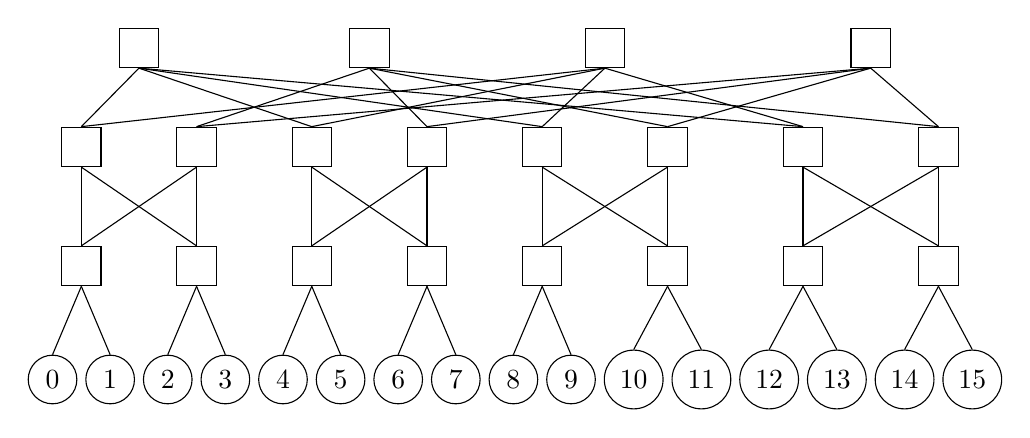
\begin{tikzpicture}[
        every node/.style={node distance=10mm and 1mm},
        server/.style={circle, draw=black, node distance=10mm and 1mm},
        switch/.style={rectangle, draw=black, minimum size=.5cm},
    ]

    % Servers
    \node[server]      (S1)                       {0};
    \node[server]      (S2)        [right=of S1]  {1};
    \node[server]      (S3)        [right=of S2]  {2};
    \node[server]      (S4)        [right=of S3]  {3};
    \node[server]      (S5)        [right=of S4]  {4};
    \node[server]      (S6)        [right=of S5]  {5};
    \node[server]      (S7)        [right=of S6]  {6};
    \node[server]      (S8)        [right=of S7]  {7};
    \node[server]      (S9)        [right=of S8]  {8};
    \node[server]      (S10)       [right=of S9]  {9};
    \node[server]      (S11)       [right=of S10] {10};
    \node[server]      (S12)       [right=of S11] {11};
    \node[server]      (S13)       [right=of S12] {12};
    \node[server]      (S14)       [right=of S13] {13};
    \node[server]      (S15)       [right=of S14] {14};
    \node[server]      (S16)       [right=of S15] {15};

    % \node[text width=2cm] at (-1.4, 0.05)  {Servers};

    % % VMs
    % \node[vm]      (V1)        [below=of S1]  {};
    % \node[vm]      (V2)        [below=of S1, left=of V1]  {};
    % \node[vm]      (V3)        [below=of S1, right=of V1]  {};

    % \node[vm]      (V4)        [below=of S8]  {};
    % \node[vm]      (V5)        [below=of S8, left=of V4]  {};
    % \node[vm]      (V6)        [below=of S8, right=of V4]  {};

    % \node[vm]      (V7)        [below=of S15]  {};
    % \node[vm]      (V8)        [below=of S15, left=of V7]  {};
    % \node[vm]      (V9)        [below=of S15, right=of V7]  {};

    % \node[text width=0.8cm] at (-2, -.86)  {VNFs};
    % \node [between=V1 and V4] {\large ...};
    % \node [between=V6 and V8] {\large ...};

    % \node[text width=0.8cm] at (-2, .86)  {Edge};
    \node[] 		 (H1) 		 [above=of S1] {};
    \node[] 		 (H2) 		 [between=S1 and S2] {};
    \node[] 		 (H3) 		 [between=S3 and S4] {};
    \node[] 		 (H4) 		 [between=S5 and S6] {};
    \node[] 		 (H5) 		 [between=S7 and S8] {};
    \node[] 		 (H6) 		 [between=S9 and S10] {};
    \node[] 		 (H7) 		 [between=S11 and S12] {};
    \node[] 		 (H8) 		 [between=S13 and S14] {};
    \node[] 		 (H9) 		 [between=S15 and S16] {};

    \node[switch]      (E1)        [at = (H1 -| H2)] {};
    \node[switch]      (E2)        [at = (H1 -| H3)] {};
    \node[switch]      (E3)        [at = (H1 -| H4)] {};
    \node[switch]      (E4)        [at = (H1 -| H5)] {};
    \node[switch]      (E5)        [at = (H1 -| H6)] {};
    \node[switch]      (E6)        [at = (H1 -| H7)] {};
    \node[switch]      (E7)        [at = (H1 -| H8)] {};
    \node[switch]      (E8)        [at = (H1 -| H9)] {};

    % Aggregate
    % \node[text width=0.8cm] at (-2, 1.67)  {Aggregation};
    \node[switch]      (A1)        [above=of E1] {};
    \node[switch]      (A2)        [above=of E2] {};
    \node[switch]      (A3)        [above=of E3] {};
    \node[switch]      (A4)        [above=of E4] {};
    \node[switch]      (A5)        [above=of E5] {};
    \node[switch]      (A6)        [above=of E6] {};
    \node[switch]      (A7)        [above=of E7] {};
    \node[switch]      (A8)        [above=of E8] {};

    % Core
    % \node[text width=0.8cm] at (-2, 2.42)  {Core};
    \node[switch]      (C1)        [above=of A1,  between=A1 and A2]  {};
    \node[switch]      (C2)        [above=of A3,  between=A3 and A4]  {};
    \node[switch]      (C3)        [above=of A5,  between=A5 and A6]  {};
    \node[switch]      (C4)        [above=of A7,  between=A7 and A8]  {};

    %Lines
    % \draw[-] (V1.north)  -- (S1.south);
    % \draw[-] (V2.north)  -- (S1.south);
    % \draw[-] (V3.north)  -- (S1.south);

    % \draw[-] (V4.north)  -- (S8.south);
    % \draw[-] (V5.north)  -- (S8.south);
    % \draw[-] (V6.north)  -- (S8.south);

    % \draw[-] (V7.north)  -- (S15.south);
    % \draw[-] (V8.north)  -- (S15.south);
    % \draw[-] (V9.north)  -- (S15.south);

    \draw[-] (S1.north)  -- (E1.south);
    \draw[-] (S2.north)  -- (E1.south);
    \draw[-] (S3.north)  -- (E2.south);
    \draw[-] (S4.north)  -- (E2.south);
    \draw[-] (S5.north)  -- (E3.south);
    \draw[-] (S6.north)  -- (E3.south);
    \draw[-] (S7.north)  -- (E4.south);
    \draw[-] (S8.north)  -- (E4.south);
    \draw[-] (S9.north)  -- (E5.south);
    \draw[-] (S10.north) -- (E5.south);
    \draw[-] (S11.north) -- (E6.south);
    \draw[-] (S12.north) -- (E6.south);
    \draw[-] (S13.north) -- (E7.south);
    \draw[-] (S14.north) -- (E7.south);
    \draw[-] (S15.north) -- (E8.south);
    \draw[-] (S16.north) -- (E8.south);

    \draw[-] (E1.north)  -- (A1.south);
    \draw[-] (E2.north)  -- (A2.south);
    \draw[-] (E3.north)  -- (A3.south);
    \draw[-] (E4.north)  -- (A4.south);
    \draw[-] (E5.north)  -- (A5.south);
    \draw[-] (E6.north)  -- (A6.south);
    \draw[-] (E7.north)  -- (A7.south);
    \draw[-] (E8.north)  -- (A8.south);

    \draw[-] (E1.north)  -- (A2.south);
    \draw[-] (E2.north)  -- (A1.south);
    \draw[-] (E3.north)  -- (A4.south);
    \draw[-] (E4.north)  -- (A3.south);
    \draw[-] (E5.north)  -- (A6.south);
    \draw[-] (E6.north)  -- (A5.south);
    \draw[-] (E7.north)  -- (A8.south);
    \draw[-] (E8.north)  -- (A7.south);

    \draw[-] (A1.north)  -- (C1.south);
    \draw[-] (A1.north)  -- (C3.south);
    \draw[-] (A2.north)  -- (C2.south);
    \draw[-] (A2.north)  -- (C4.south);
    \draw[-] (A3.north)  -- (C1.south);
    \draw[-] (A3.north)  -- (C3.south);
    \draw[-] (A4.north)  -- (C2.south);
    \draw[-] (A4.north)  -- (C4.south);
    \draw[-] (A5.north)  -- (C1.south);
    \draw[-] (A5.north)  -- (C3.south);
    \draw[-] (A6.north)  -- (C2.south);
    \draw[-] (A6.north)  -- (C4.south);
    \draw[-] (A7.north)  -- (C1.south);
    \draw[-] (A7.north)  -- (C3.south);
    \draw[-] (A8.north)  -- (C2.south);
    \draw[-] (A8.north)  -- (C4.south);
\end{tikzpicture}

\end{document}